\documentclass[12pt,a4paper]{article}

\usepackage[utf8]{inputenc}
\usepackage[ngerman]{babel}
\usepackage[T1]{fontenc}
\usepackage{amsmath}
\usepackage{amsfonts}
\usepackage{amssymb}
\usepackage{graphicx}
\usepackage[left=2cm,right=2cm,top=2cm,bottom=2cm]{geometry}
\usepackage{multicol}
\usepackage{booktabs}
\usepackage[hidelinks]{hyperref}
\usepackage{tikz}
\usepackage{pgfplots}
\usepackage{blindtext}
\usepackage{array}
\usepackage{multirow}
\usepackage{bigdelim}
\usepackage{colortbl}
\usepackage{fancyhdr} 
\usepackage{tabularx}
\usepackage{pgfplots}
\usepackage{xcolor}
\usepackage{color}
\usetikzlibrary{decorations.text}
\usetikzlibrary{tikzmark}
\pagestyle{fancy} 
	\fancyhf{} 
	\fancyhead[L]{
\includegraphics[scale=0.05]{Bilder/dhbw.png}} 
	\fancyhead[C]{\slshape WLAN} 
	\fancyhead[R]{\slshape LaTeX Version}

\usepackage{helvet}
\renewcommand{\familydefault}{\sfdefault}

\newcolumntype{Z}{>{\centering\let\newline\\\arraybackslash\hspace{0pt}}X}
\author{\slshape Robin Rausch, Florian Maslowski, Ozan Akzebe}
\title{WLAN}
\date{\slshape \today}

\begin{document}
\maketitle
\tableofcontents
\newpage

\section{WLAN Intro}
	Standards for wireless communication
	Akronyme:
	\begin{description}
		\item[BSS:] Basic Service set: Ist ...
		\item[STA:] Station 
		\item[IBSS:] Infrastruktur Basic Service Set: Ist ... 
	\end{description}

\section{Funknetz}
	Base station-> Base station controller (BSC): verbindet Base stations-> Mobile switching center (MSC): verbindet BSC mit Festnetz (PSTN) und Internet-> externes Netzwerk
	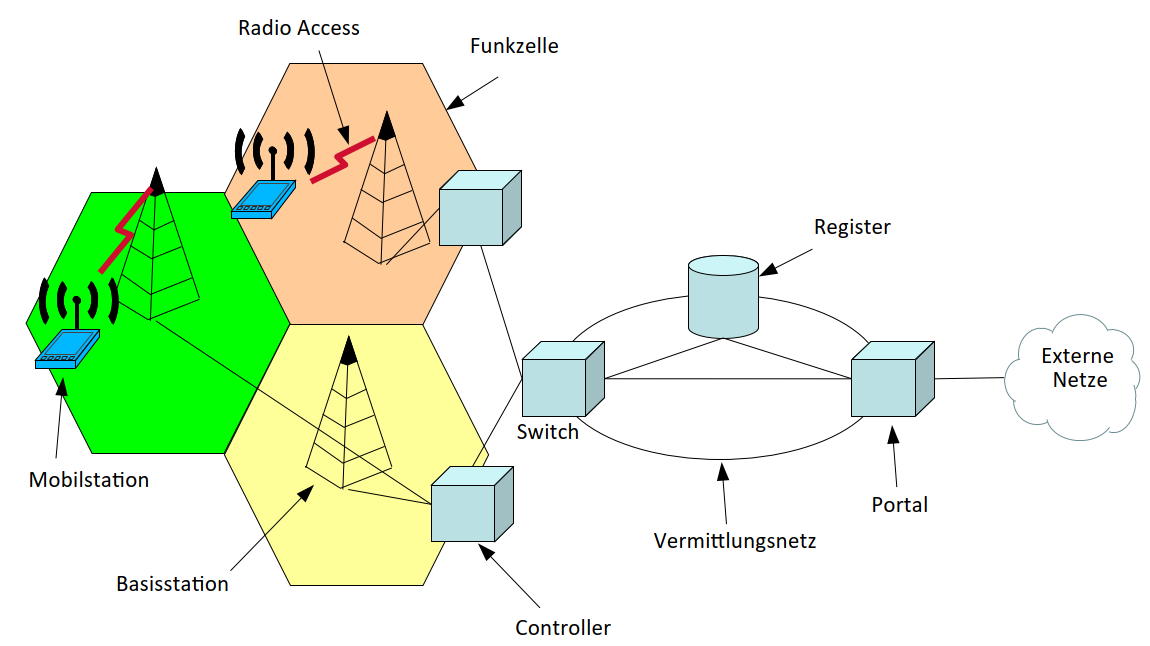
\includegraphics[width=\textwidth]{Bilder/Funknetz.png}

	\subsection*{Handover vs. Roaming}
		Handover ist Übergabe von Accesspoint zu Accesspoint im selben Subnetz (Layer 2).\\
		Roaming ist Übergabe von Accesspoint zu Accesspoint in anderes Subnetz (Layer 3).
	
\section{Modi}
	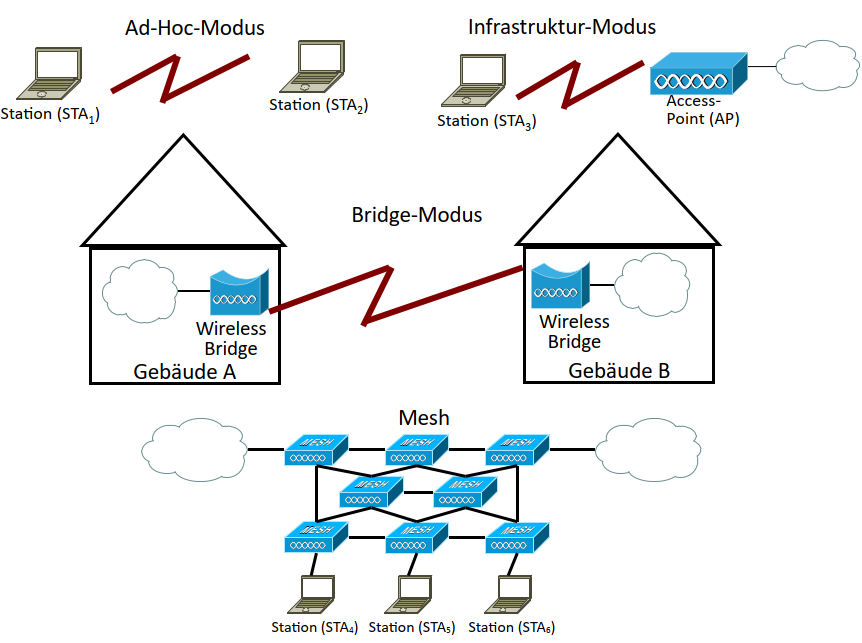
\includegraphics[width=0.5\textwidth]{Bilder/Funkmodi.png}
	\subsection*{Ad-Hoc}

	\subsection*{Infrastruktur}

	\subsection*{Bridge}

	\subsection*{Mesh}

\section{Standards}
	\begin{description}
		\item[WPA1:] 
		\item[WPA2:]
		\item[WPA3:]    
	\end{description}

\section{Sicherheit}


\section{Mobile IP}


\end{document}